\documentclass[oneside]{article}

\usepackage{blindtext} % dummy text
\usepackage{graphicx} % for figures
\usepackage{color} % for colored text
\usepackage{colortbl} % for colored text
\usepackage{float} % for forcing figure placement
\usepackage[breakable]{tcolorbox} % for text box
\usepackage{enumerate} % for bullet point lists
\usepackage{setspace} % line spacing
\usepackage{soul} % strike through
\usepackage[normalem]{ulem} % strike through keeping emphasis standard
\usepackage{cancel} % diagonal strike through
\usepackage[margin=1in]{geometry} % margins

\usepackage[sc]{mathpazo} % Use the Palatino font
\usepackage[T1]{fontenc} % Use 8-bit encoding that has 256 glyphs
% \linespread{1.05} % Line spacing - Palatino needs more space between lines
\usepackage{microtype} % Slightly tweak font spacing for aestheticsgins
\usepackage[small,labelfont=bf,up,up]{caption} % Custom captions under/above floats in tables or figures
\usepackage{booktabs} % Horizontal rules in tables
\usepackage{amsmath} % Text in equations
\usepackage{titlesec} % Allows customization of titles
\usepackage{titling} % Customizing the title section
\usepackage[hidelinks]{hyperref} % For hyperlinks in the PDF

\usepackage{algorithm2e}

\usepackage{tikz}
\usetikzlibrary{shapes.geometric, arrows, positioning, decorations.markings, shapes.multipart}   
\usepackage{standalone}

\usepackage{subcaption} % for subfigures side by side
\captionsetup[subfigure]{singlelinecheck=false} % to put (a) and (b) at the top-left of subfigures

\usepackage[shortlabels]{enumitem} % customized lists (shortlabels
                                % necessary to have i., ii., etc., in enumerate)
\setlist[itemize]{noitemsep} % Make itemize lists more compact

\usepackage{abstract} % Allows abstract customization
\renewcommand{\abstractnamefont}{\normalfont\bfseries} % Set the "Abstract" text to bold
\renewcommand{\abstracttextfont}{\normalfont\small\itshape} % Set the abstract itself to small italic text

\usepackage{fancyhdr} % Headers and footers
\pagestyle{fancy} % All pages have headers and footers
\fancyhead{} % Blank out the default header
\fancyfoot{} % Blank out the default footer
\fancyhead[C]{Mendes et al. $\bullet$ December 2023 $\bullet$ bio{\color{red}R}$\chi$ve} % Custom header text
\fancyfoot[RO,LE]{\thepage} % Custom footer text



\usepackage{natbib}
\bibliographystyle{apalike}

\usepackage{libertine}

\setlength\columnsep{20pt}

%----------------------------------------------------------------------------------------
%	TITLE SECTION
%----------------------------------------------------------------------------------------

\setlength{\droptitle}{-4\baselineskip} % Move the title up

%\pretitle{\begin{center}\Huge\bfseries} % Article title formatting
%\posttitle{\end{center}} % Article title closing formatting

\title{How to validate a Bayesian evolutionary model} % Article title
%LM: strictly speaking, we're 'validating' the inference machinery.
%% Validating a model involves epistemic considerations that are, as far as I understand, outside the scope of this paper.
\author{\textsc{F\'{a}bio K. Mendes$^{1\dagger*}$}, \textsc{Remco Bouckaert$^{2\dagger}$},\\
\textsc{Luiz M. Carvalho$^{3\dagger}$}, \textsc{Alexei J. Drummond$^{4}$} \\
\small $^1$Department of Biology, Washington University in St. Louis\\
\small $^2$School of Computer Science, The University of Auckland\\
\small $^3$Escola de Matem\'{a}tica Aplicada, Fundaç\~{a}o Getulio Vargas\\
\small $^4$School of Biological Sciences, The University of Auckland\\
\small
\href{mailto:f.mendes@auckland.ac.nz}{$^*$Corresponding author: f.mendes@auckland.ac.nz}\\
{\small $^\dagger$Authors contributed equally to this work}
% \href{mailto:f.mendes@auckland.ac.nz}{another.email@auckland.ac.nz}
%\and % Uncomment if 2 authors are required, duplicate these 4 lines if more
%\textsc{Jane Smith}\thanks{Corresponding author} \\[1ex] % Second author's name
%\normalsize University of Utah \\ % Second author's institution
%\normalsize \href{mailto:jane@smith.com}{jane@smith.com} % Second author's email address
}
\date{\today} % Leave empty to omit a date

\renewcommand{\figurename}{Supplementary Figure}
\renewcommand{\tablename}{Supplementary Table}

\doublespacing

\begin{document}

\maketitle

\begin{center}
    \Large Supplementary Material
\end{center}

\newpage
% \section{Additional validation examples and guidelines}

\section{Validating a phylogenetic Brownian motion simulator}

In this section we focus on validating a simulator for the phylogenetic Brownian motion model (``PhyloBM''; \citealp{felsenstein73}).
As explained in the main text, our goal is to verify that the expected value of certain summary statistics (given a specific combination of parameter values) falls within its $\alpha$-confidence intervals approximately $\alpha$\% of the time.
We will build confidence intervals about statistics calculated from several PhyloBM samples of size 10,000, and then ask if the ``population'' value of  a statistic -- given by the parameters of the multivariate normal sampling distribution -- is contained within its confidence interval frequently enough.

For summary statistics, we pay attention to the trait value's (i) species mean, (ii) species variance, (iii) among-species covariance, and (iv) among-species correlation coefficient.
Supplementary figure \ref{supfig:bmsimcis} shows one hundred confidence intervals for each of these statistics, under multivariate normal $\text{MVN}(\boldsymbol{y_0},r\boldsymbol{T})$, where $\boldsymbol{y_0}=\{0,0,0\}$, $r=0.1$ and $\boldsymbol{T}$ is given by the tree in Fig. 2 in the main text.
Supplementary table \ref{suptab:bmsimcis} summarizes how often each statistic fell within its 95\%-confidence interval.
These results indicate the PhyloBM simulator produces appropriate confidence intervals and behaves as expected.

\begin{figure}
  \centering
  \includestandalone[width=14cm]{../figures/phylobm_exp_vcv_cis}
  \caption{One hundred 95\%-confidence intervals (blue and red lines) built for four different summary statistics, when validating a phylogenetic Brownian motion model simulator.
    Red lines represent intervals that do not contain the value expected under the MVN sampling distribution defined by a bifurcating three-taxon phylogenetic tree.
    Summary statistics include each leaf's character-value mean (top row) and variance (second row from the top), as well as pairwise (leaf) character-value co-variances (third row from the top) and correlations (bottom row).}
  \label{supfig:bmsimcis}
\end{figure}

\begin{table}[h]
  \caption{The number of times $k$ that a summary statistic was contained within its corresponding 95\%-confidence interval.
    Each statistic was calculated from 100 datasets of size 10,000 simulated under the PhyloBM model described in the text and in Box 1 in the main text.}
  \label{suptab:bmsimcis}
  \centering
  \begin{tabular}{ ccc }
    \hline
    Statistic & Species $s$ (and $v$)& $k$\\
    \hline  
    \rowcolor{gray!10}                      & A & 95\\
    \rowcolor{gray!10} $\text{E}[y_s]$      & B & 97\\
    \rowcolor{gray!10}                      & C & 98\\
                                            & A & 93\\
                       $\text{Var}[y_s]$    & B & 97\\
                                            & C & 97\\
    \rowcolor{gray!10}                      & A and B & 95\\
    \rowcolor{gray!10}$\text{Cov}[y_s,y_v]$ & A and C & 95\\
    \rowcolor{gray!10}                      & B and C & 97\\
                                            & A and B & 96\\
                      $\text{Cor}[y_s,y_v]$ & A and C & 96\\
                                            & B and C & 97\\
    \hline
  \end{tabular}
\end{table}

\newpage
\section{Model validation with rejection sampling: a simple example}
\label{sec:supp_toy}

In this section, we experiment with a simple hierarchical Gaussian (toy) model to further examine the effect of rejection sampling in coverage validation and
rank-uniformity validation (RUV).
This experiment is motivated by results described in the main text, namely, the model in scenario 3 (Fig. 1, with extreme rejection sampling) passing coverage validation but not RUV.

Let us devise the following data-generating process for obtaining different levels of model misspecification:

\begin{align*}
 \mu & \sim \operatorname{Normal}\left(0, 1\right)T[t, ],\\
  y_1, \ldots, y_K & \overset{\text{iid}}{\sim} \operatorname{Normal}\left(\mu, 1\right),
\end{align*}
where $K$ is the sample size, and notation $T[, t]$ indicates the distribution is truncated \textbf{below} at $t \in \mathbb{R}$, i.e.,
\begin{equation*}
    \pi_{t}(\mu) = \frac{\phi(\mu)}{1 - \Phi(t)} \mathbb{I}(\mu > t).
\end{equation*}
and $\phi$ and $\Phi$ are the pdf and CDF of a standard normal, respectively.
Here, $\mu$ and $y_1, \ldots, y_K$ correspond to $\theta_i$ and $d_i$ in Fig. 4 (main text), respectively.

Inference is then done under the misspecified model
\begin{align*}
 \mu & \sim \operatorname{Normal}\left(0, 1\right),\\
  y_1, \ldots, y_K & \overset{\text{i.i.d.}}{\sim} \operatorname{Normal}\left(\mu, 1\right).
\end{align*}
It is well-known that:
\begin{equation}
\label{eq:toy_normal_posterior}
    \mu \mid y_1, \ldots, y_K \sim \operatorname{Normal}\left( \frac{\sum_{k = 1}^K y_k}{K + 1},  \frac{1}{K + 1} \right),
\end{equation}
i.e., the posterior is known in closed-form so MCMC is not required and one can sample directly and independently from it.
One can thus control how extreme the model misspecification will be during inference by increasing $t$.
Here we explore $t =  \{0, 1, 1.5\}$ and $K = \{5, 10 , 50\}$ in order to show how the method behaves in various misspecification scenarios.
We ran $n=1000$ replications of the experiment, draw $200$ i.i.d. samples directly from the posterior in (\ref{eq:toy_normal_posterior}).

The resulting rank histograms (Supplementary Fig.~\ref{supfig:ruv_normal_toy}) show how the posterior consistently underestimates the true mean, as indicated by a pattern of ranks bunching up towards the right-hand side of the histogram.
The pattern is clearer in situations where the evidence in the data is weaker (e.g., when $K$ is small), and the effect of the prior on the posterior is stronger.
Moreover, the misspecification becomes more apparent the larger $t$ is, that is, the more extreme the misspecification becomes.

It is worth noting a couple of things.
First, unlike what we observed and reported for the model in the main text, coverage validation does suggest an incorrectly specified model for certain combinations of $t$ and $K$ (Supplementary Table 2).
Second, when the truncation is less extreme ($t = 0$) and there is a substantial amount of data ($K = 50$), RUV fails to detect any problems.
This is an important insight about validation protocols: their sensitivity is context-dependent, and responds to the combination of model and data regime.

\begin{figure}[!ht]
   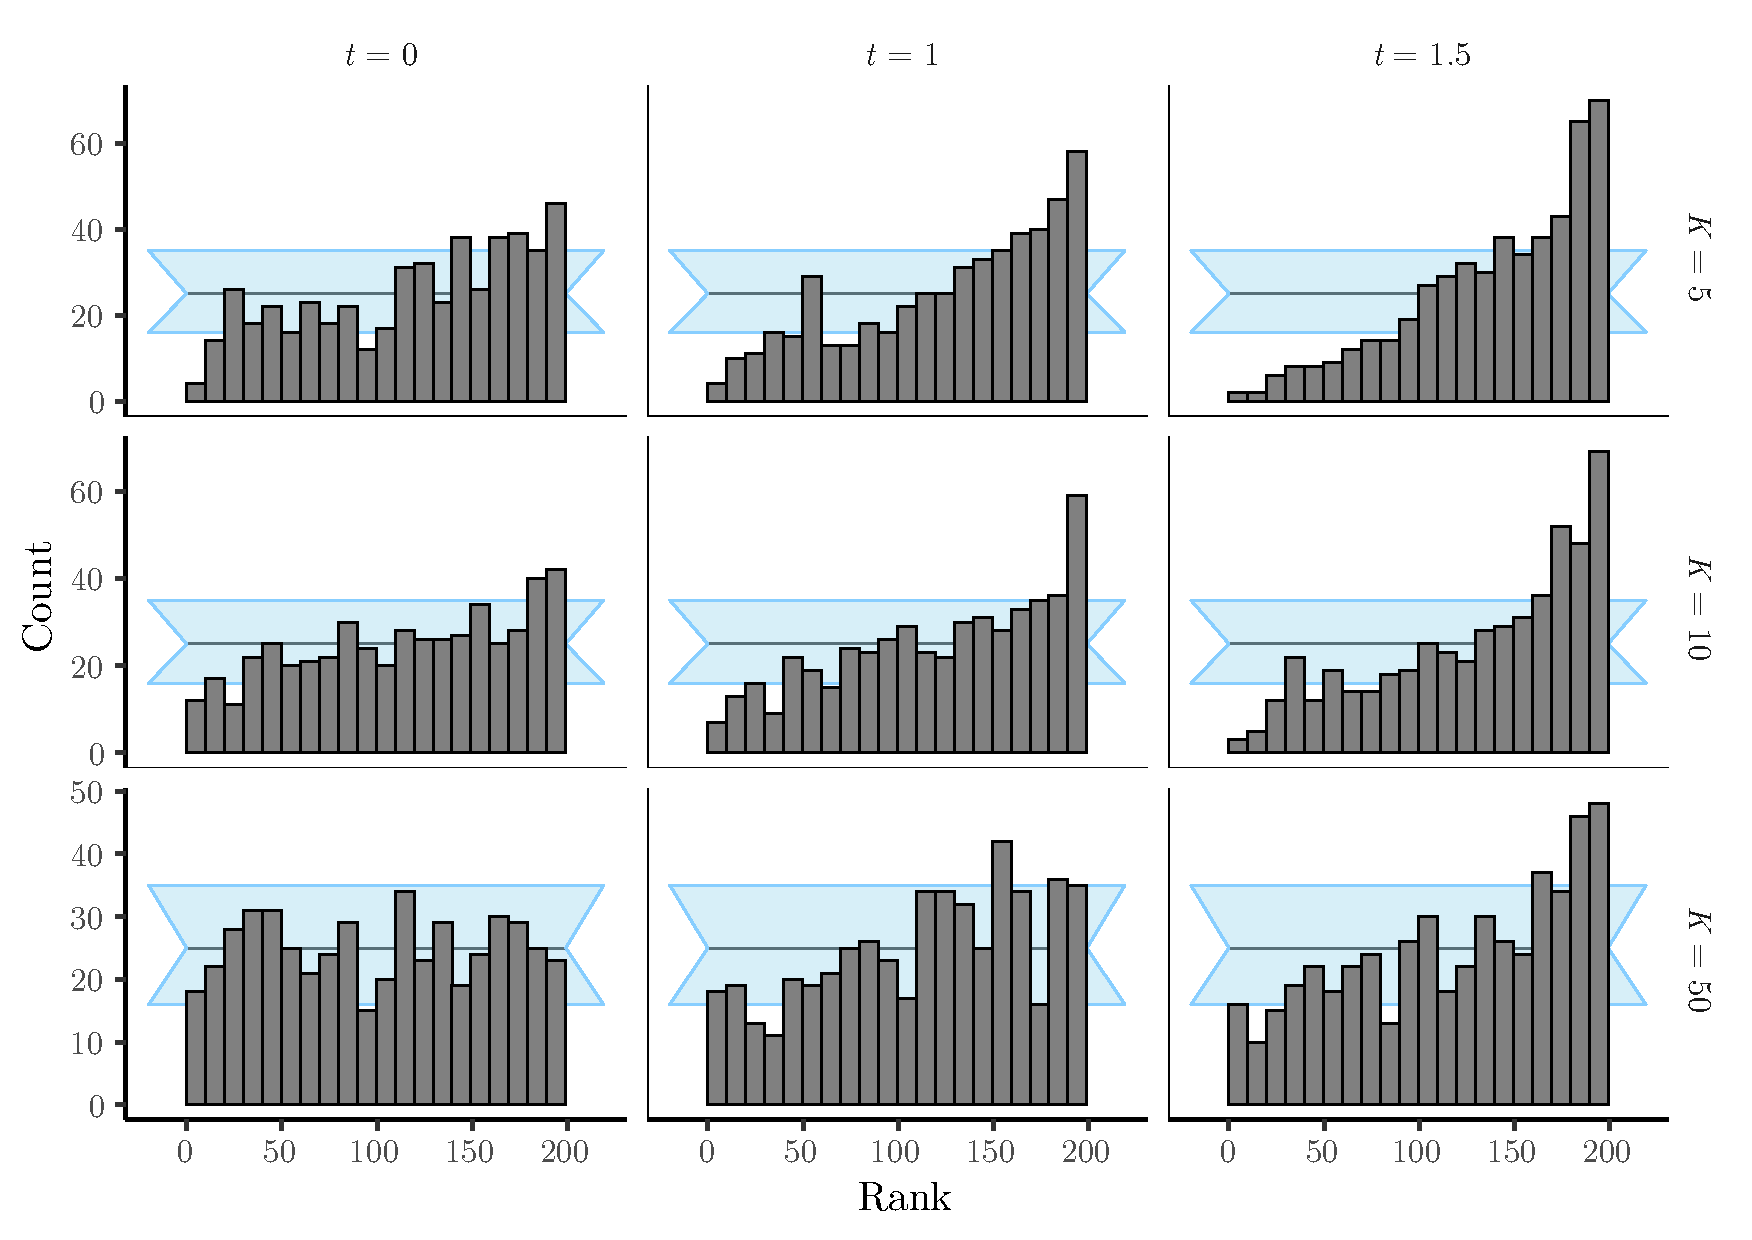
\includegraphics[width=\linewidth]{../figures/sbc_normal_manual.pdf}
  \caption{Rank-uniformity validation (RUV) of the hierarchical Gaussian toy model.
  We show the rank histograms in three misspecification scenarios ($t$
  is 0.0, 1.0 or 1.5) and three data regimes ($K$ is 5, 10 or 50).
  Results are based on $n=1000$ replicates of $L= 200$ i.i.d. draws each.
  Horizontal black lines shows the expected count for each rank (the same for all ranks due to uniformity), and the light-blue bands represent the 95\%-confidence interval for the counts.
    }
  \label{supfig:ruv_normal_toy}
\end{figure}

\begin{table}[!h]
\caption{Coverage results for the 95\%-HPD under the hierarchical Gaussian toy model.
For each combination of truncation ($t$) and data set size ($K$), we show the estimated coverage over $n=1000$ replicates, and whether the coverage procedure passes.
A pass is determined according to table 2 in the main text.
}
\centering
\begin{tabular}{cccc}
  \hline
  Truncation ($t$) & Number of observations ($K$) & Estimated coverage & Pass \\
  \hline
  \rowcolor{gray!10} 0   & 5                      & 0.93               & No     \\
  \rowcolor{gray!10} 1   & 5                      & 0.92               & No     \\
  \rowcolor{gray!10} 1.5 & 5                      & 0.90               & No     \\
                     0   & 10                     & 0.95               & Yes    \\
                     1   & 10                     & 0.91               & No     \\
                     1.5 & 10                     & 0.91               & No     \\
  \rowcolor{gray!10} 0   & 50                     & 0.96               & Yes    \\
  \rowcolor{gray!10} 1   & 50                     & 0.93               & No     \\
  \rowcolor{gray!10} 1.5 & 50                     & 0.93               & No     \\
  \hline
\end{tabular}
\end{table}

\newpage
\section{Validating a phylogenetic model with respect to a phylogenetic tree parameter, $\Phi$}
\label{sec::app::ruv_topology}

Our goal is to evaluate if an inferential implementation of model $\mathcal{M}$, $\text{I}[\mathcal{M}]$, is well-calibrated and correct.
In this section, we will focus on one critical parameter of $\mathcal{M}$: the phylogenetic tree $\Phi$.
We will pay special attention to $\Phi$ while carrying out coverage validation and the RUV procedure.
In practice, this amounts to computing the coverage of $\Phi$ and the rank distribution of this parameter in comparison to its posterior samples.

What feature of $\Phi$ should one use when calculating coverage and ranks?
Because of the nature of tree space, summarizing and comparing phylogenetic trees with univariate measures is not a trivial task.
The key to an effective validation effort is to choose a functional that reflects relevant estimators of the quantity of interest, in our case, $\Phi$.
Fortunately, it is possible to exploit the metric nature of tree space and compute quantities both from a sampled phylogenetic tree $\phi$ -- i.e., the ``true'' tree simulated during the validation process -- as well as distances with respect to a reference phylogeny $\phi_0$.
We summarize some of these distances in supplementary table \ref{suptab:dists}.

\begin{table}[h]
  \caption{Metrics (functionals) for investigating model correctness in phylogenetic tree space. $\phi$ is a (phylogenetic tree) sample of $\Phi$, sampled from a tree model (e.g., a Yule process).
  $\phi_0$ is a reference tree to which $\phi$ and its posterior samples (see Algorithm 1 and the RUV section in the main text) are being compared, with respect to any of the metrics in the table.
  \textcolor{brown}{For the KC metric, the parameter ($\omega$) controls the balance between topological and branch length information and was set at $\omega = 1/2$.} }
  \label{suptab:dists}
  \centering
  \begin{tabular}{ l|c|c }
    \hline
    \multicolumn{1}{c|}{Metric} & Notation & Ref. \\
    \hline  
    \rowcolor{gray!10}The largest branch length in $\phi$ & $\text{LB}(\phi)$ & N/A\\
    The length of $\phi$ (the sum of all branch lengths) & $\text{LEN}(\phi)$ & N/A\\
    % \rowcolor{gray!10}The length of the external branch leading to taxon $s_1$ & $\text{T}_1(\phi)$ & N/A\\
    \rowcolor{gray!10}The difference between the largest and smallest branch length of $\phi$ & $\text{R}(\phi)$ & N/A\\
    The Robinson-Foulds distance between $\phi$ and $\phi_0$ & $\text{RF}_0(\phi)$ & \citep{rf81}\\
    \rowcolor{gray!10}The Kendall-Coljin distance between $\phi$ and $\phi_0$ & $\text{KC}_0(\phi;\omega)$ & \citep{Kendall2016}\\
    The Billera-Holmes-Vogtman distance between $\phi$ and $\phi_0$ & $\text{BHV}_0(\phi)$ & \citep{Billera2001}\\
    \hline
  \end{tabular}
\end{table}

In the case of tree-space distance metrics, we must slightly modify our RUV procedure (Algorithm 1).
The key difference is the sampling of a reference phylogenetic tree, $\phi_0$, prior to the simulation of the $n$ i.i.d. $\Phi$ samples, $\boldsymbol{\phi}=\{\phi_i: 1 \leq i \leq n\}$.
Given a reference tree $\phi_0$, each sampled $\phi_i$ and all of its $L$ posterior MCMC samples are then compared to $\phi_0$ with respect to a chosen distance metric.
It is the evaluated distance metric that will underlie the ranking of $\phi_i$ relative to its posterior MCMC samples.
Once ranks are computed, RUV proceeds as usual.
   
\RestyleAlgo{ruled}
\SetKwComment{Comment}{/* }{ */}

\begin{algorithm}[h]
  \DontPrintSemicolon
  \SetKwFunction{GenRefTree}{GenerateRefTree}
  \SetKwFunction{InitH}{InitializeHyperparameters}
  \SetKwFunction{SampleNT}{SampleNonTreeParameters}
  \SetKwFunction{SampleTree}{SampleTree}
  \SetKwFunction{SampleData}{SampleData}
  \SetKwFunction{Distance}{CalculateDistance}
  \SetKwFunction{MCMC}{MCMC}
  \SetKwFunction{Rank}{GetRank}
  \SetKwFunction{Pass}{IsRankDistributionUniform}
  \caption{Algorithm for carrying out a rank-uniformity validation procedure with respect to the phylogenetic tree parameter $\Phi$.
    Parameters $\boldsymbol{\theta}$ include both the tree parameter, $\theta_\Phi$, and non-tree (scalar) parameters, $\boldsymbol{\theta}_{\text{s}}$.
    Data $\boldsymbol{d}$ represents the output of an evolutionary process taking place along the phylogenetic tree (e.g., a continuous-time Markov chain modeling DNA substitutions).}
  \label{alg:sbcphylo}
  $n \gets 100$\; \Comment*[r]{Number of data sets to simulate}
  $\theta_{\mathcal{H}} \gets$ \InitH{}\; \Comment*[r]{Hyperparameters initialized to constant values}
  $\boldsymbol{\theta}_0 \gets$ \SampleNT{$\theta_{\mathcal{H}}$}\; \Comment*[r]{$\boldsymbol{\theta}_0 \sim f_\Theta(\cdot)$, with $\boldsymbol{\theta}_0 = \{\theta_{\Phi,0},\boldsymbol{\theta}_{\text{s},0}\}$}
  $\phi_0 \gets$ \SampleTree{$\theta_{\Phi,0}$}\; \Comment*[r]{$\phi_0 \sim f_{\Phi|\Theta_{\Phi}}(\cdot|\Theta_\Phi=\theta_{\Phi,0})$}
  \For{$i \gets 1$ \KwTo $n$} {
    $\boldsymbol{\theta}_i \gets$ \SampleNT{$\theta_{\mathcal{H}}$}\; \Comment*[r]{$\boldsymbol{\theta}_i \sim f_\Theta(\cdot)$, with $\boldsymbol{\theta}_i = \{\theta_{\Phi,i},\boldsymbol{\theta}_{\text{s},i}\}$}
    $\phi_i \gets$ \SampleTree{$\theta_{\Phi,i}$}\; \Comment*[r]{$\phi_i \sim f_{\Phi\mid \Theta_\Phi}(\cdot|\Theta_\Phi=\theta_{\Phi,i})$}
    $d_i \gets$ \SampleData{$\phi_i,\boldsymbol{\theta}_{\text{s},i}$}\; \Comment*[r]{$d_i \sim f_{D\mid \Phi,\boldsymbol{\Theta}_\text{s}}(\cdot|\Phi=\phi_i,\boldsymbol{\Theta}_{\text{s}}=\boldsymbol{\theta}_{\text{s},i})$}
    $\boldsymbol{\theta}'_i \gets$ \MCMC{$f_{D|\boldsymbol{\Theta}}(d_i|\boldsymbol{\Theta}=\boldsymbol{\theta}_i)f_{\boldsymbol{\Theta}}(\boldsymbol{\theta}_i)$}\; \Comment*[r]{$\boldsymbol{\theta}'_i = \{\boldsymbol{\theta}_i^j: 1 \leq j \leq L\}$, where $L$ is the number of MCMC samples}
    $\bar{\delta}_i \gets$ \Distance{$\phi_0, \phi_i$}\; \Comment*[r]{According to a distance metric of choice}
    $\boldsymbol{\delta}_i^j \gets$ \Distance{$\phi_0, \phi_i^j$}\; \Comment*[r]{$\boldsymbol{\delta}_i = \{\delta_i^j: 1 \leq j \leq L\}$}
    $r_i \gets$ \Rank($\bar{\delta}_i, \boldsymbol{\delta}_i^j$)\; \Comment*[r]{$r_i = \sum\limits_{j=1}^L \mathbb{I}(\delta^j_i < \bar{\delta_i})$}
  }
  \If{\Pass{$\boldsymbol{r}$}}{
    \Return \textbf{true}
  }
  \Else {
    \Return \textbf{false}
  }
  \label{alg:sbc}
\end{algorithm}

  % \begin{enumerate}
  %   \setcounter{enumi}{-1}

  % \item Generate a reference tree from the prior $\bar{\Phi}_0  \sim f_T(\Phi | \boldsymbol \theta_\Phi)$; 

  %   \textbf{for} each iteration in 1:N, \textbf{do}:
    
  % \item Generate $\bar{\Phi} \sim f_T(\Phi | \boldsymbol \gamma)$;
  % \item Compute the distance $\bar{\delta} = d_\sigma(\bar{\Phi},\bar{\Phi}_0)$ according to the metric of choice;
  % \item Generate some (aligment) data $\tilde{d} \sim f_{D\mid\Phi}(d | \bar{\Phi}, \boldsymbol\alpha)$;
  % \item Draw\footnote{Sometimes approximately, using MCMC or variational methods.} $\boldsymbol \Phi_s = \{\Phi_s^{(1)}, \Phi_s^{(2)}, \ldots, \Phi_s^{(L)}\}$ from the posterior $f_{\Phi\mid D}(\Phi | \tilde{d})$;
  % \item Compute distances $\boldsymbol \delta_s = \{ \delta_1, \delta_2, \ldots, \delta_L \}$  with $\delta_i = d_\sigma(\Phi_s^{(i)}, \bar{\Phi}_0)$;
  % \item Compute the rank $r(\boldsymbol\delta_s, \bar{\delta}) = \sum\limits_{i=1}^L \mathbb{I}(\delta_i < \bar{\delta})$.
  % \end{enumerate}

\begin{figure}
  \centering
  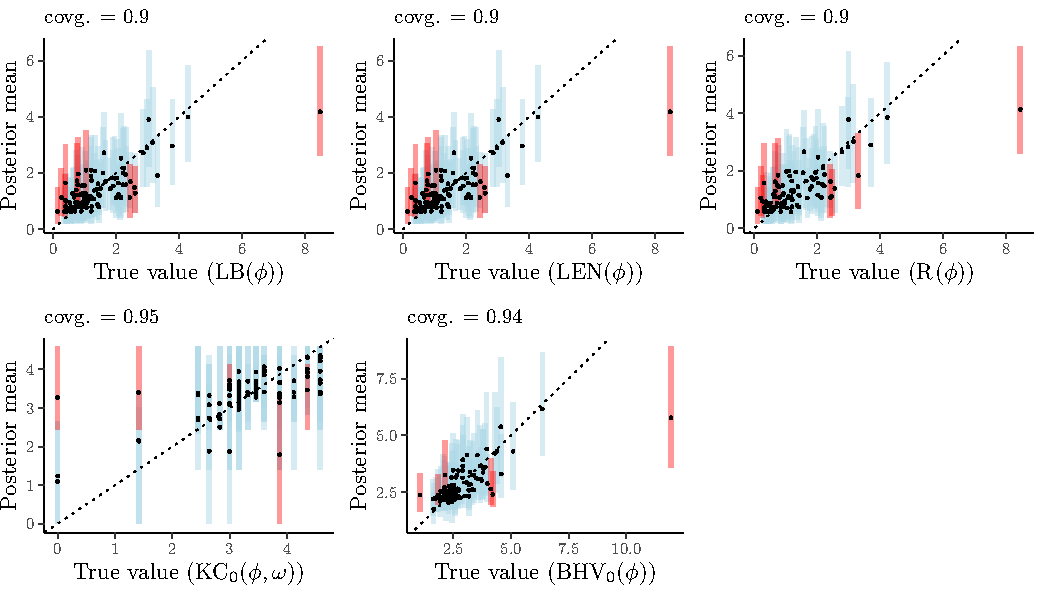
\includegraphics[width=\linewidth]{../figures/tree_stats_coverage_manual.pdf}
   \caption{Coverage validation of a phylogenetic model, focusing on the phylogenetic tree parameter (see Supplementary Table \ref{suptab:dists} for a description of the different distance metrics).}
   \label{supfig:treecov}
 \end{figure}
 
\begin{figure}
  \centering
  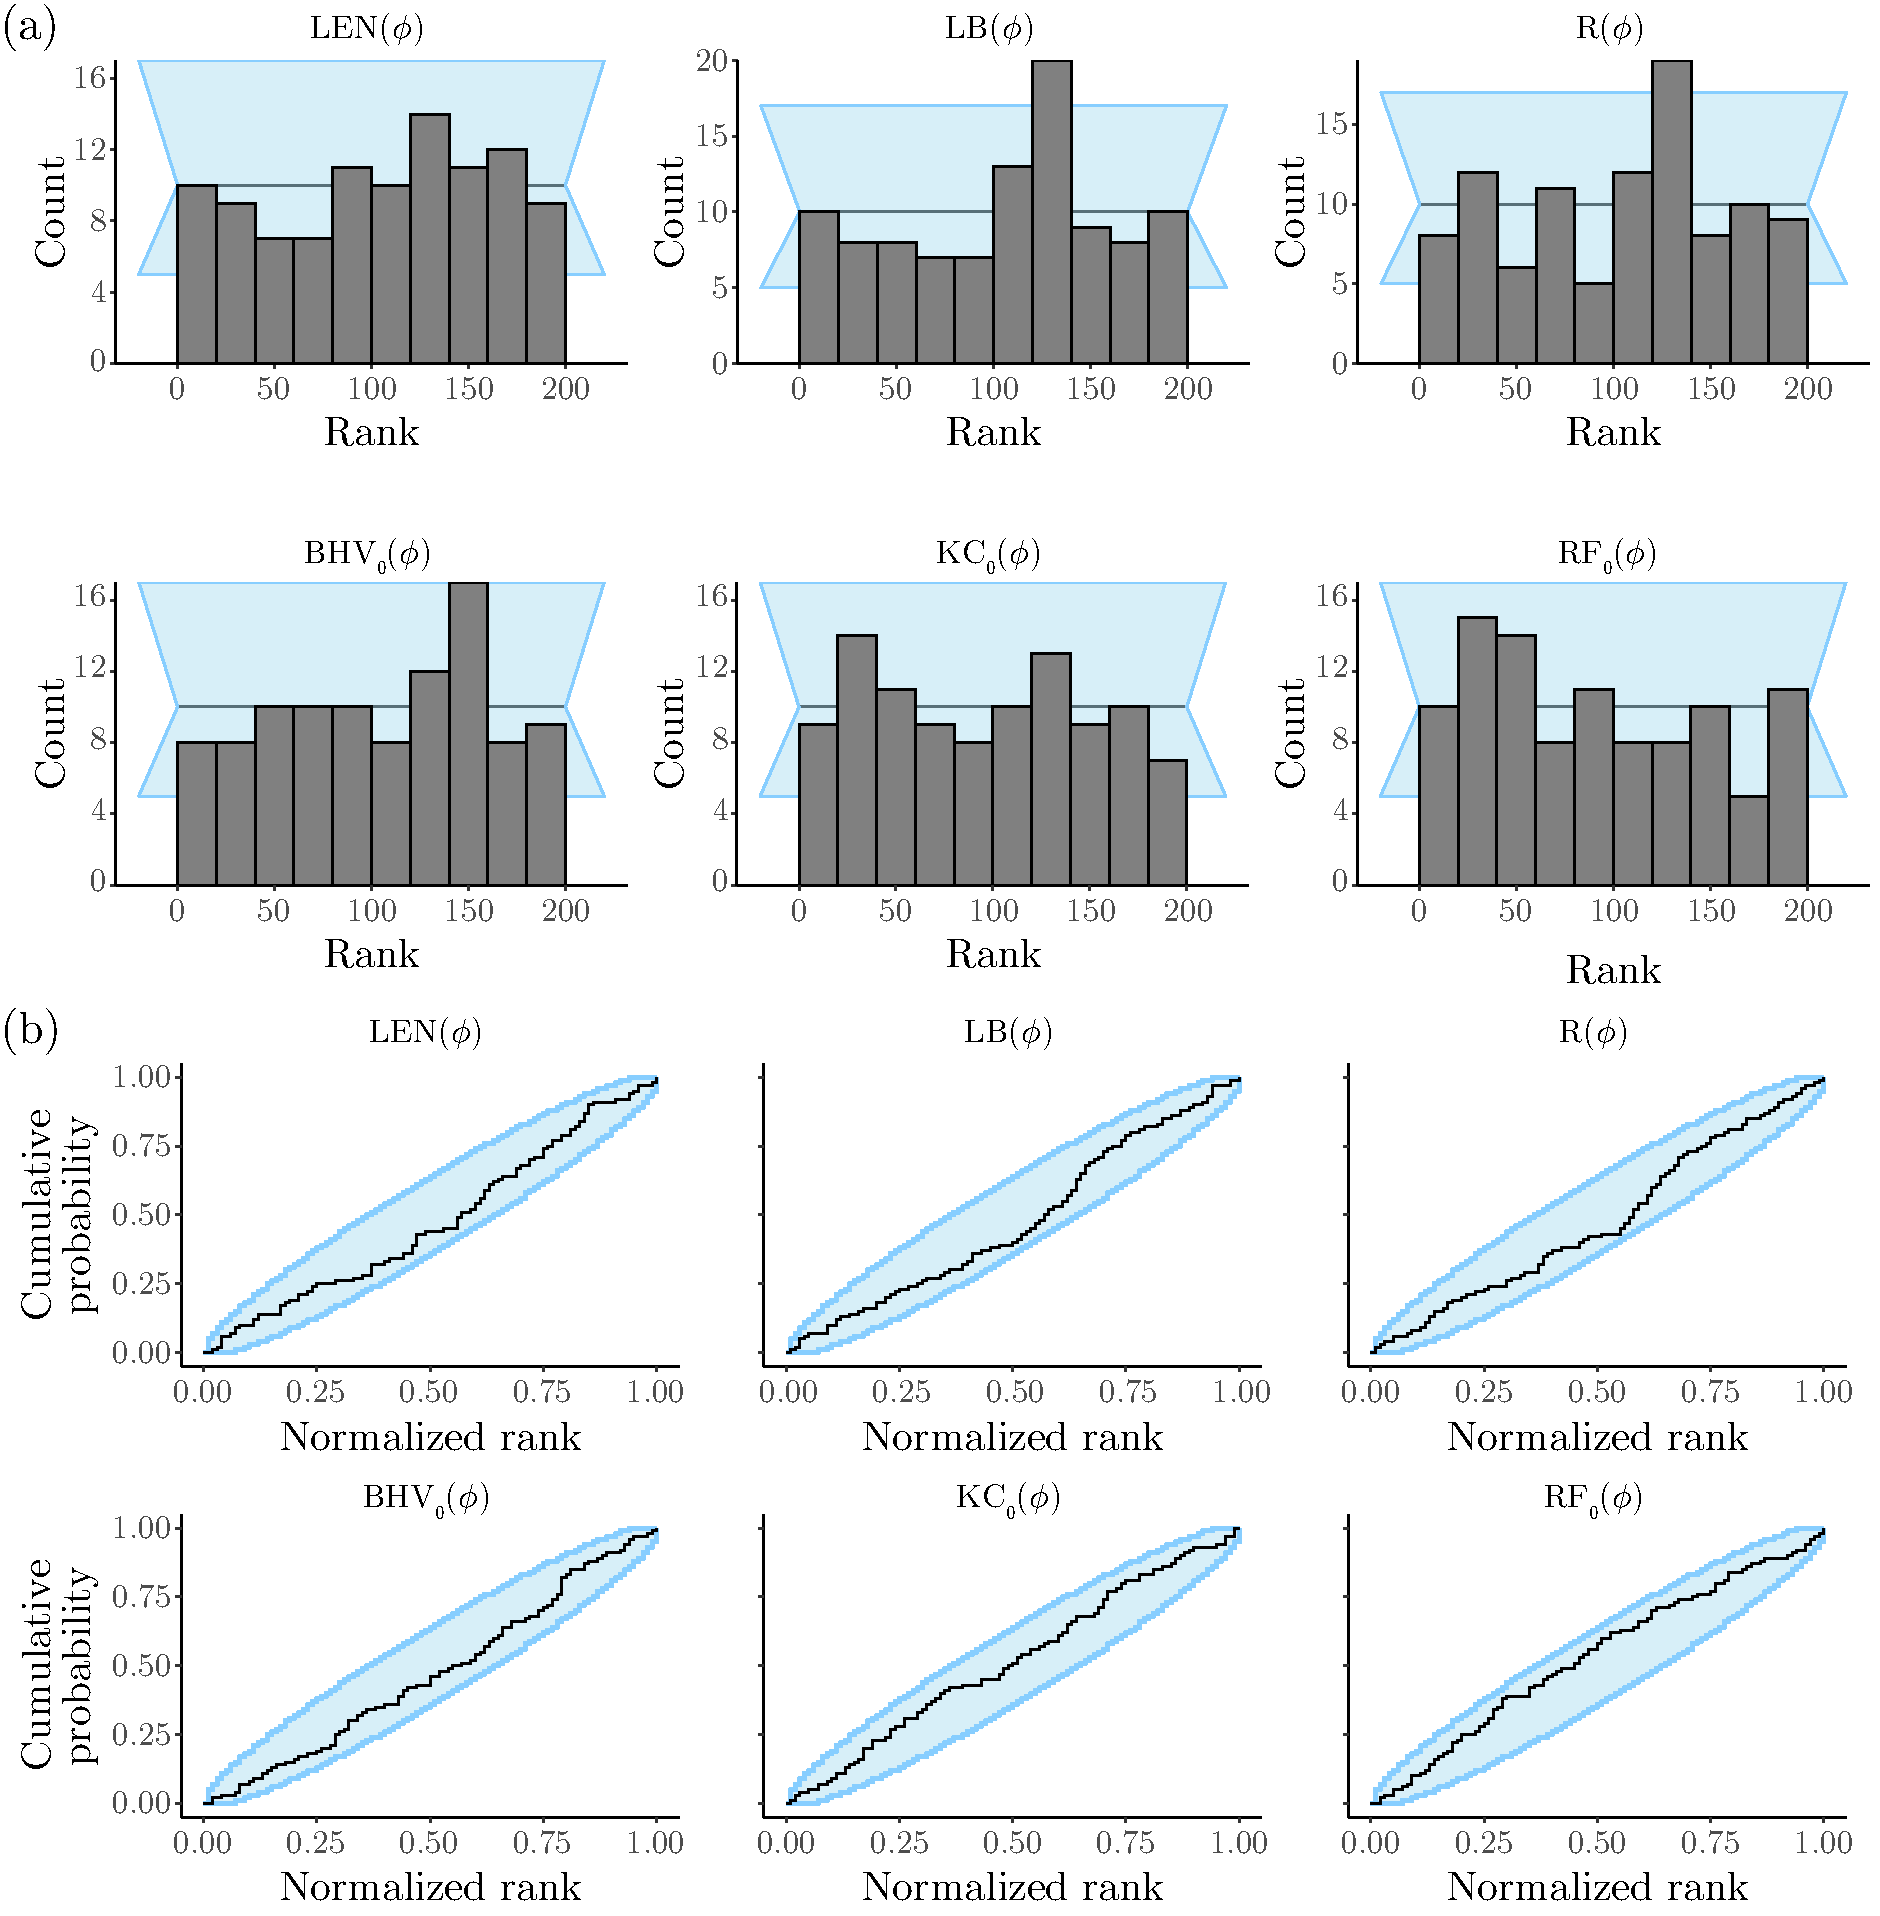
\includegraphics[width=\linewidth]{../figures/ruv_coalescent_manual.pdf}
  % \vspace{0pt}
  % \begin{subfigure}[t]{\textwidth}
  %   \caption{}
  %   \centering
  %   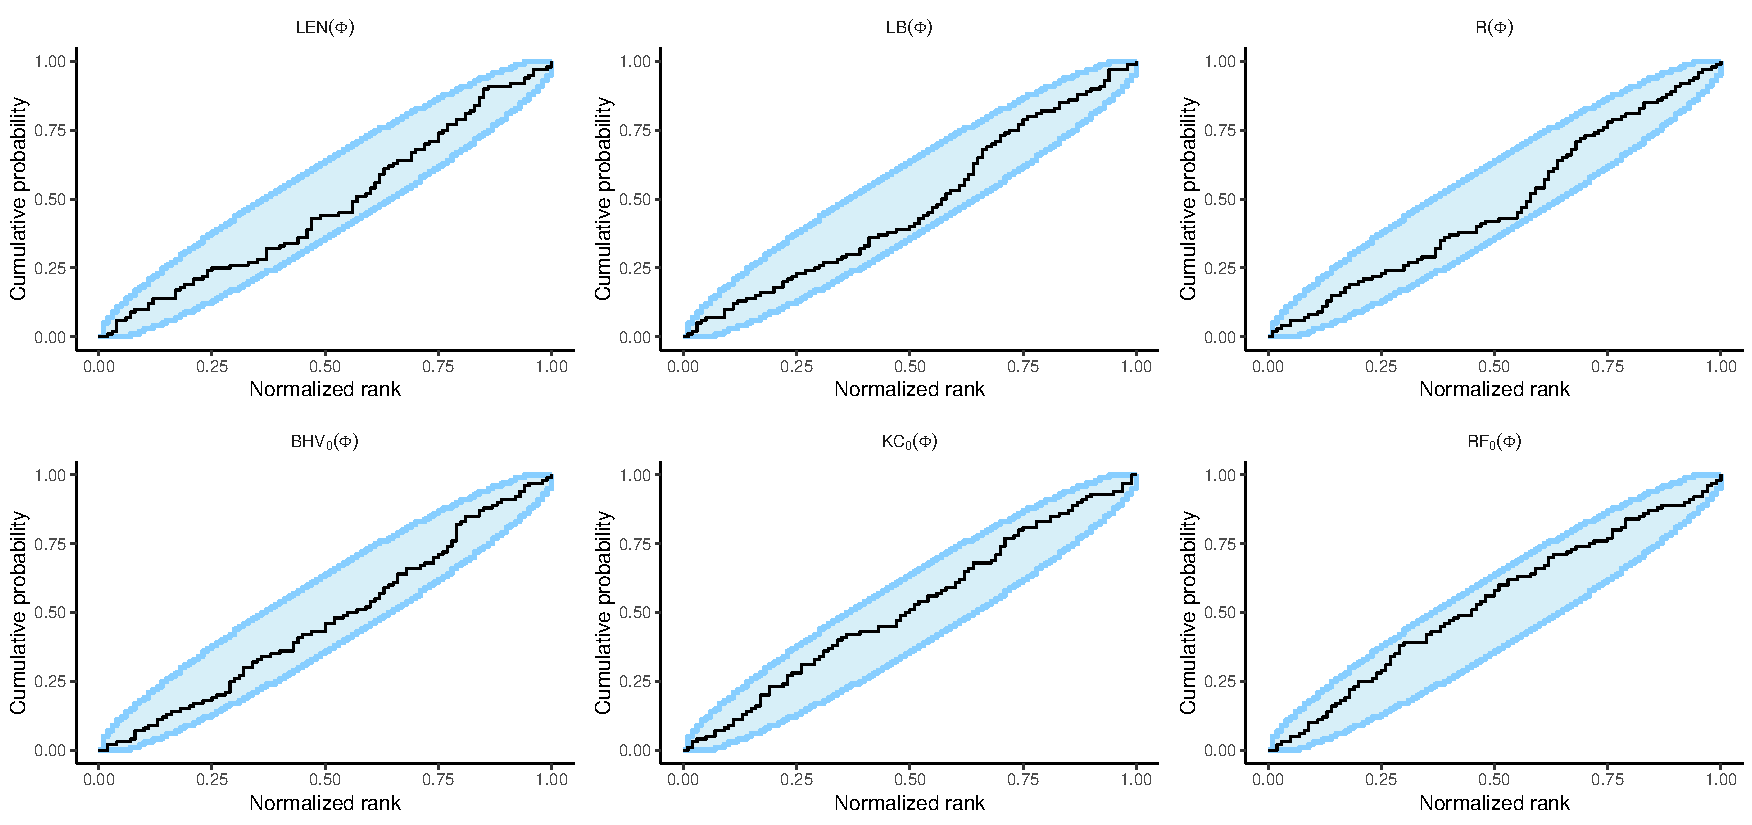
\includegraphics[scale=0.5]{../figures/ruv_coalescent_ecdfs.pdf} 
  % \end{subfigure}
  % \vspace{0pt}
  % \hspace{1cm}
  % \begin{subfigure}[t]{\textwidth}
  %   \caption{}
  %   \centering
  %   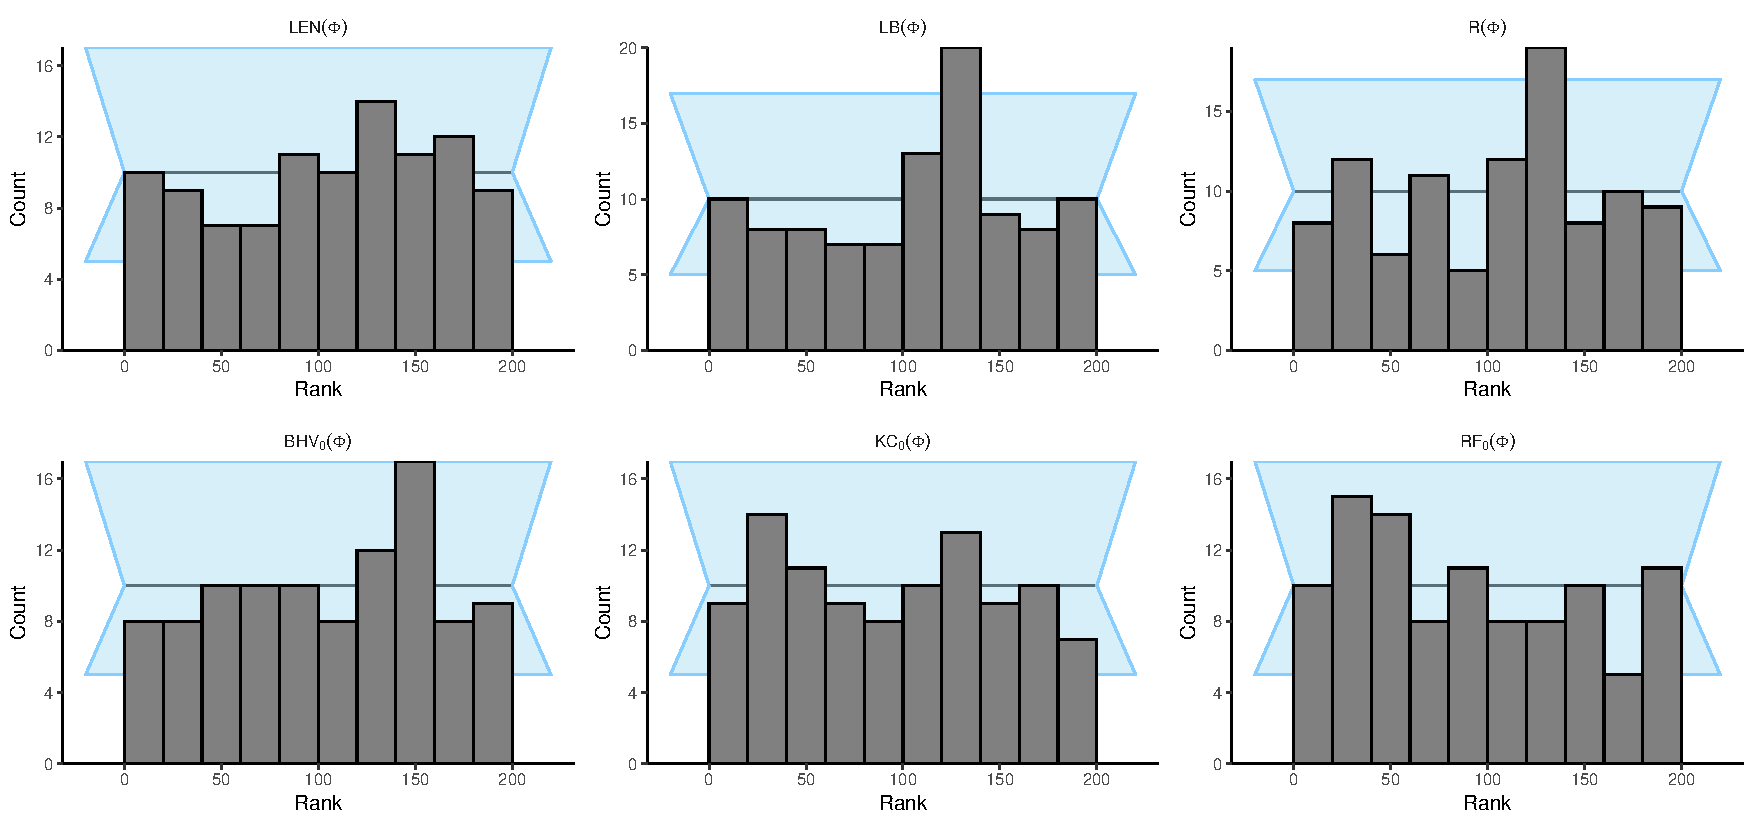
\includegraphics[scale=0.5]{../figures/ruv_coalescent_histograms.pdf}    
  % \end{subfigure}
  % \hfill
   \caption{Rank-uniformity validation (RUV) of a phylogenetic model, focusing on the phylogenetic tree parameter (see Supplementary Table \ref{suptab:dists} for a description of the different distance metrics).
     (a) Rank distribution for each metric.
     (b) Empirical cumulative distribution function (ECDF) for each metric.
   }
   \label{supfig:ruv}
\end{figure}

% \begin{figure}
%  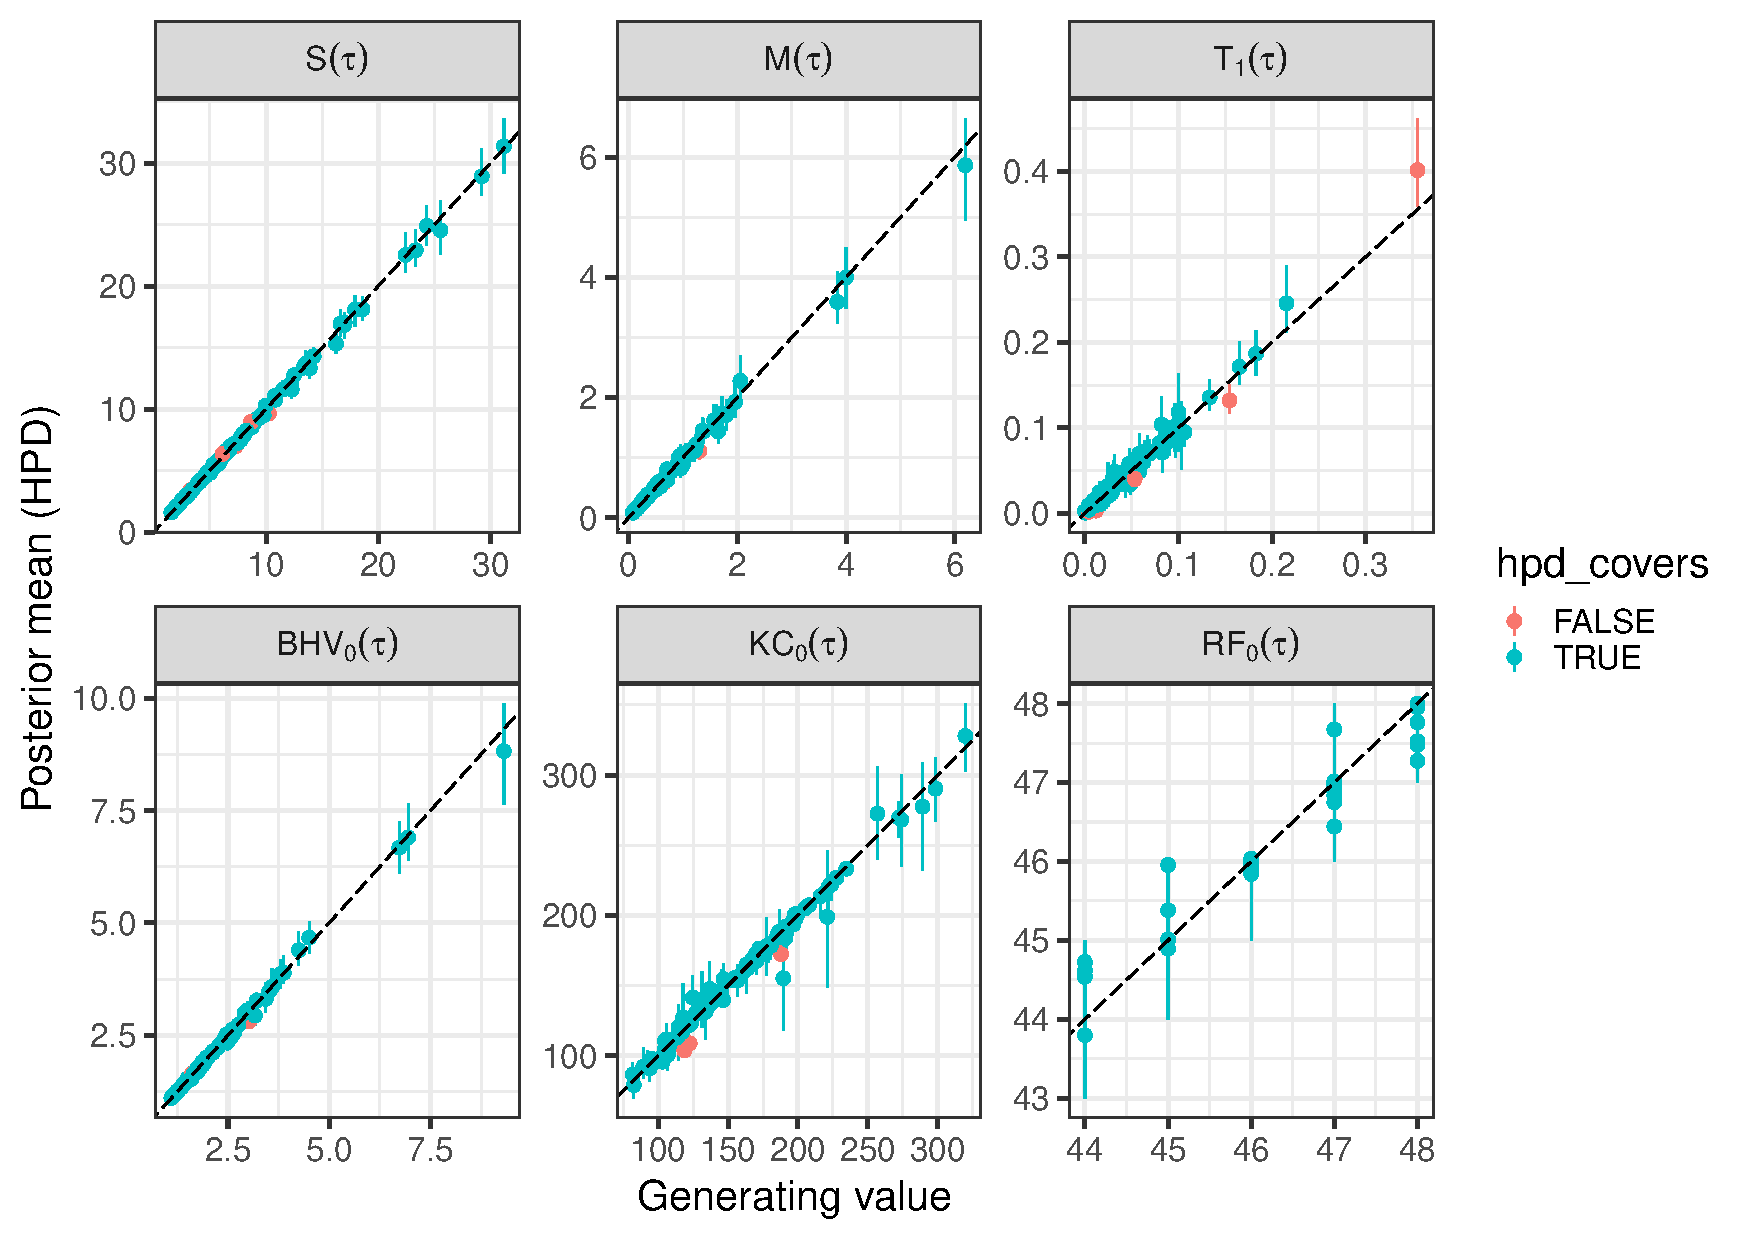
\includegraphics[width=\textwidth]{../figures/coverage.pdf}
%     \caption{Coverage for different functionals in validation experiment.
%         % rank-uniformity validation.
%       Posterior means are represented by point and 95\% HPDs by bars.
%       Red dots and lines show intervals that failed to include the
%       generating value, whilst blue ones show those that did include
%       the simulated ``truth''.}
%   \label{supfig:phylo_calibration}
% \end{figure}

Supplementary figures \ref{supfig:treecov} and \ref{supfig:ruv} summarize the coverage and RUV results, respectively, for the metrics listed in supplementary table \ref{suptab:dists}, when the model is the simple Kingman's coalescent.
The model consists of a single five-taxon phylogenetic tree parameter, $\Phi$, assuming a known effective population size of 1.0.

We can first verify that our model implementation is well-calibrated with respect to the phylogenetic tree parameter, as shown by appropriate 95\%-HPD-coverage statistics over the different tree metrics (Supplementary Fig. \ref{supfig:treecov}).
The evidence for implementation correctness is enhanced by observing that the ranks for the different metrics are (approximately) uniformly distributed, lying inside their confidence bands (Supplementary Fig. \ref{supfig:ruv}a), and their corresponding ECDFs also lie well inside their confidence ellipses (Supplementary Fig. \ref{supfig:ruv}b).
% Supplementary figure \ref{supfig:phylo_calibration} shows that the HPDs do cover the
% generating metrics with probability compatible with what is expected
% theoretically.
% In this instance, the tests would fail to detect problems with the algorithm.
% These plots can be supplemented with a table showing attained coverage and binomial confidence intervals for this quantity.
% A further advantage of graphically investigating coverage is that one can identify consistent areas for which estimation fails -- e.g. high/low simulated values of a given variable.

\newpage
\section{Proof for coverage validation}
 \label{appendix::sec:proofs}

In this section we provide a mathematical argument that coverage-based validation is sound, i.e., that sampling from the prior, simulating data and then using the same prior for computing the posterior should give Bayesian credible intervals (BCIs) with nominal frequentist coverage.

For a number $n$ of replicates, simulate parameter
  values $\theta_i$, and then given those values, simulate data $d_i$:

\begin{align*}
\theta_i & \sim f_\Theta(\cdot), \\
d_i & \sim f_{D|\Theta}(\cdot | \Theta=\theta_i).
\end{align*}

Now for notational convenience, define $a_i := a(d_i, \alpha)$ as the HPD lower bound and, similarly, $b_i := b(d_i, \alpha)$ as the HPD upper bound.
Recall $I_{\alpha}\left(d_i\right)$ is such that:


\begin{align*}
Q_{d_i}\left(b_i\right) - Q_{d_i}\left(a_i\right) = p_1 - p_2 = \alpha,
\end{align*}

\noindent where $Q_{d}(x)$ is the posterior CDF (conditional on data $d$) and $p_1, p_2 \in (0,1)$, with $p_1 < p_2$.
A natural quantity to compute is:

\begin{align*}
S_n = n^{-1}\sum_{i=1}^n \mathbb{I}\left(\theta_i \in I_{\alpha}\left(d_i\right) \right),
\end{align*}

\noindent i.e., the attained coverage of the Bayesian intervals.

Let $F_U(x) = x$ be the CDF of a $\operatorname{Uniform(0, 1)}$ random variable. 
Now we can consider what happens when the number of simulations grows, i.e., the limit $\lim_{n \to \infty} S_n$.
We may re-write the limit as:

\begin{align*}
\lim_{n \to \infty} S_n &= \lim_{n \to \infty} n^{-1}\sum_{i=1}^n \mathbb{I}\left(\theta_i \in I_{\alpha}\left(d_i\right) \right),\\
&=  \lim_{n \to \infty} n^{-1}\sum_{i=1}^n \left\{ \mathbb{I}\left(\theta_i \leq b_i \right) - \mathbb{I}\left(\theta_i \leq a_i \right) \right\},\\
&=  \lim_{n \to \infty} n^{-1}\sum_{i=1}^n \mathbb{I}\left(\theta_i \leq b_i \right) -  n^{-1}\sum_{i=1}^n\mathbb{I}\left(\theta_i \leq a_i \right),\\
&=  \lim_{n \to \infty} n^{-1}\sum_{i=1}^n \mathbb{I}\left(Q_{d_i}^{-1}\left(\theta_i\right) \leq p_1 \right) -   \lim_{n \to \infty} n^{-1}\sum_{i=1}^n\mathbb{I}\left(Q_{d_i}^{-1}\left(\theta_i\right) \leq p_2 \right),\\
&= F_U(p_1) - F_U(p_2) = \alpha,
\end{align*}

\noindent where the last line follows from the fact that the CDF of $\theta_i$ is uniformly distributed on $(0, 1$) (Theorem 1 in \citealp{Cook06}) and almost sure convergence of the ECDF to the true CDF due to the  Glivenko-Cantelli theorem~\cite[page 275]{Billingsley1986}.

\newpage
\section{Other supplementary figures}
\label{appendix::sec:supp_figures}

\begin{figure}[!ht]
   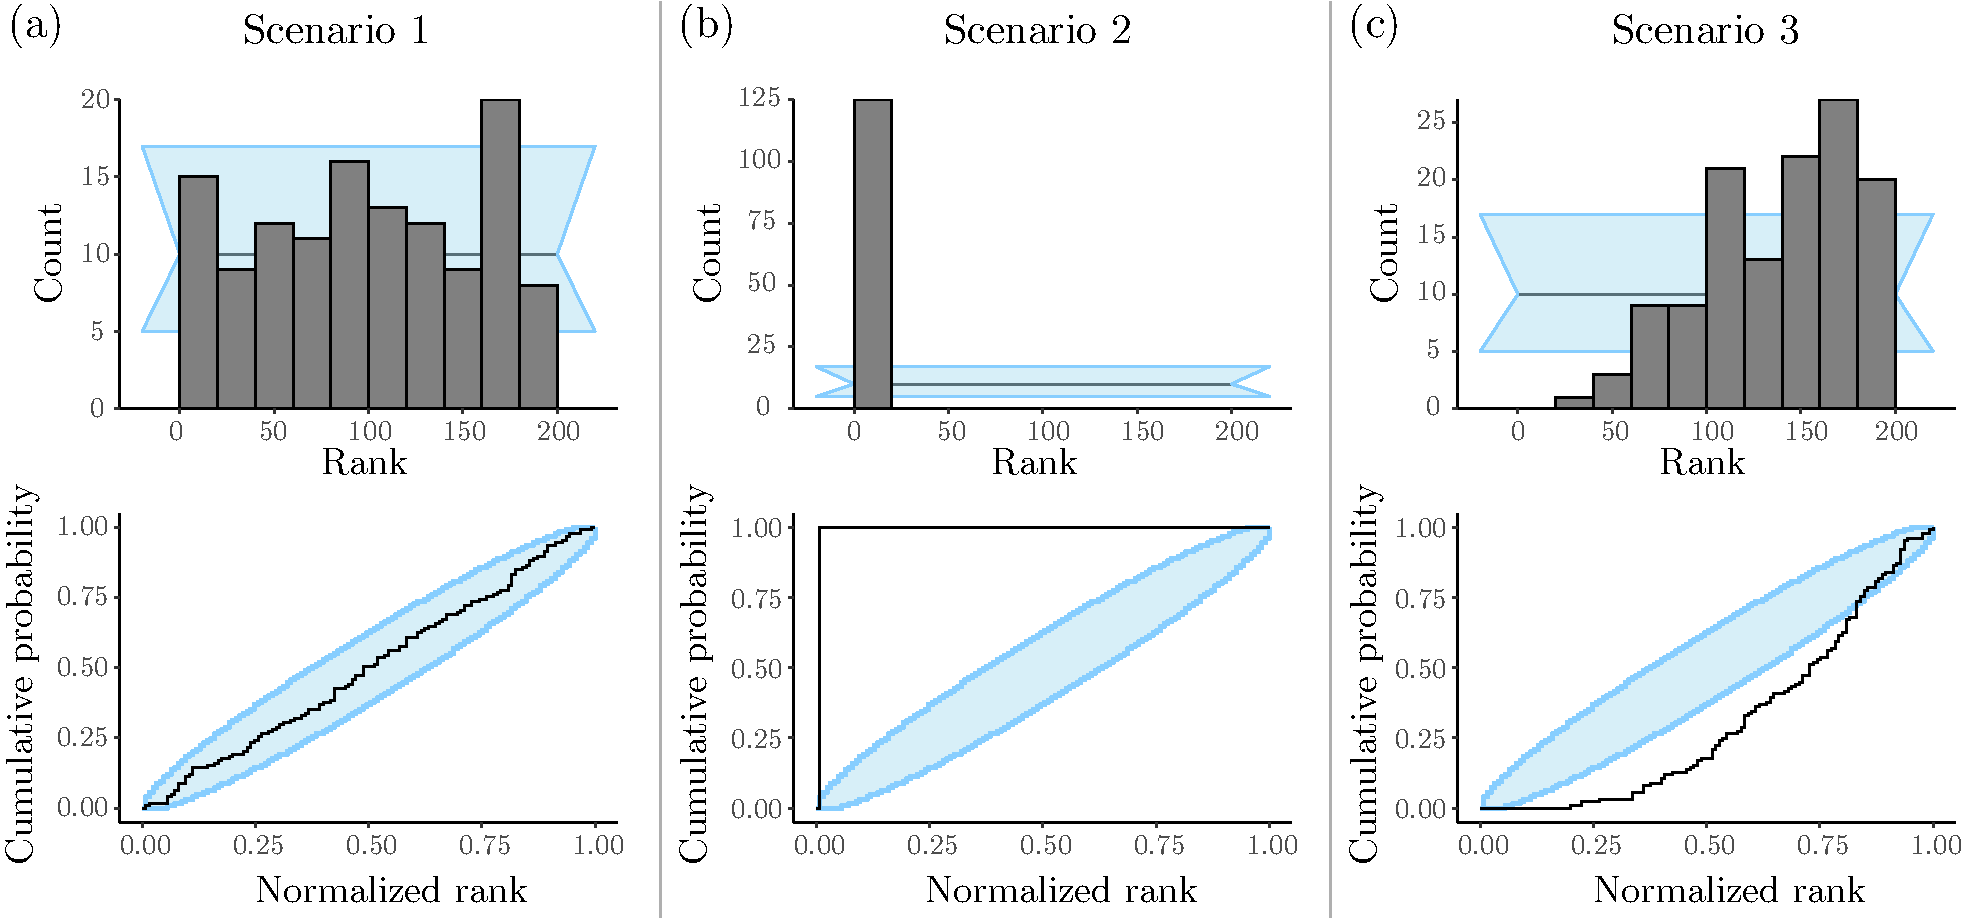
\includegraphics[width=\linewidth]{../figures/sbc_Yule_lambda_manual.pdf}
  \caption{Rank-uniformity validation (RUV) of the Bayesian hierarchical model in Fig. 1 in the main text.
    Panels in the top row show the histograms of $n=100$ ranks, for parameter $\Lambda$ in each scenario, obtained after 10\% burnin and thinning of posterior samples down to 200 out of 10,000.
    Panels in the bottom row show the corresponding ECDF plots, for parameter $\Lambda$ in each scenario.
    (a) In ``Scenario 1'', the model was correctly specified, and we simulated trees with 3 to 300 taxa using rejection sampling (approximately one in ten trees were rejected).
    (b) In ``Scenario 2'', the model was incorrectly specified in inference (see main text), and we used the same data sets simulated in ``Scenario 1''.
    (c) In ``Scenario 3'', the model was correctly specified, but rejection sampling was more intense (we rejected a large number of trees, approximately 90\%, keeping those having between 100 to 200 tips).
   }
  \label{supfig:ruv_yule_lambda}
\end{figure}

\clearpage

\bibliography{refs}

\end{document}
